\documentclass{article}

% ICML 2024 Packages
\usepackage{icml2024}
\usepackage{times}
\usepackage{hyperref}
\usepackage{url}
\usepackage{amsmath}
\usepackage{amssymb}
\usepackage{graphicx}
\usepackage{booktabs}
\usepackage{algorithm}
\usepackage{algorithmic}

\icmltitlerunning{Efficient Liveness Detection via Frequency-Decoupled VAE}

\begin{document}

\twocolumn[
\icmltitle{Efficient Liveness Detection via Frequency-Decoupled \\
           Variational Autoencoder with Landmark-Only Input}

\icmlsetsymbol{equal}{*}

\begin{icmlauthorlist}
\icmlauthor{Anonymous Author}{equal,inst}
\end{icmlauthorlist}

\icmlaffiliation{inst}{Institution, Address, Country}

\icmlcorrespondingauthor{Anonymous Author}{email@domain.com}

\icmlkeywords{Liveness Detection, Variational Autoencoder, One-Class Learning, Frequency Decomposition}

\vskip 0.3in
]

\printAffiliationsAndNotice{}

\begin{abstract}
Face liveness detection is critical for preventing presentation attacks in face recognition systems. However, existing methods often require extensive labeled fake samples and computationally expensive deep networks. We propose an efficient two-stage approach that combines frequency-decoupled variational autoencoders (VAE) with landmark-only input. In Stage 1, we perform one-class learning on real samples using a novel band-split VAE that decomposes facial motion into interpretable frequency bands. Stage 2 fine-tunes the model with a small number of fake samples using either margin-based or discriminative losses. By operating solely on facial landmarks (40 points), our method achieves $89.26\%$ F1-score with significantly fewer parameters than video-based approaches. The frequency decomposition provides interpretability, revealing that fake videos exhibit distinct anomalies in different frequency bands. Our approach demonstrates that effective liveness detection is achievable with minimal supervision and computational resources.
\end{abstract}

\section{Introduction}
\label{sec:intro}

Face recognition systems are increasingly vulnerable to presentation attacks, where adversaries use photos, videos, or deepfake-generated content to spoof authentication systems~\citep{chingovska2012face, boulkenafet2015face}. Liveness detection—distinguishing live faces from fake presentations—has become essential for securing biometric systems.

Traditional liveness detection methods rely on hand-crafted features such as texture analysis~\citep{maatta2011face} or motion patterns~\citep{kollreider2007evaluating}. Recent deep learning approaches~\citep{liu2018learning, george2019deep} achieve higher accuracy but require: (1) extensive labeled datasets of both real and fake samples, (2) computationally expensive 3D CNNs or recurrent networks operating on full video frames, and (3) substantial model parameters.

We identify three fundamental limitations in existing approaches. First, \textbf{data efficiency}: most methods require large-scale labeled fake datasets, which are expensive to collect and quickly become outdated as attack methods evolve. Second, \textbf{computational efficiency}: processing full video frames with deep networks incurs high computational costs. Third, \textbf{interpretability}: deep models provide limited insight into \emph{why} a sample is classified as fake.

In this work, we propose a novel two-stage framework that addresses these limitations through three key contributions:

\textbf{(1) Landmark-only representation:} We operate exclusively on 40 facial landmark trajectories rather than raw pixels, reducing input dimensionality from $300 \times H \times W \times 3$ to $300 \times 40 \times 2$ (where 300 is temporal length). This achieves $>1000\times$ parameter reduction while preserving essential motion dynamics.

\textbf{(2) Efficient two-stage learning:} Stage 1 employs one-class learning on real samples only, learning the manifold of genuine facial motion through a variational autoencoder. Stage 2 fine-tunes with minimal fake samples (538 vs. 1088 real) using either margin-based or discriminative objectives, demonstrating that extensive fake datasets are unnecessary.

\textbf{(3) Frequency-decoupled architecture:} We introduce a band-split VAE that decomposes facial motion into three interpretable frequency bands—low (0-2Hz), band-pass (2-8Hz), and high (8-15Hz)—corresponding to head pose, speech-related motion, and micro-expressions. This decomposition enables interpretability and reveals that fake videos exhibit characteristic anomalies in specific frequency bands.

Our experiments on 234 test samples demonstrate that both proposed Stage 2 methods achieve $89.26\%$ F1-score, outperforming the Stage 1 baseline ($86.64\%$ F1) with only 538 additional fake training samples. The frequency decomposition provides actionable insights: fake videos generated by audio-driven synthesis show anomalies primarily in band-pass frequencies, while replayed videos exhibit uniform degradation across all bands.

\section{Method}
\label{sec:method}

\subsection{Overview}

Our framework consists of two stages: (1) one-class VAE pretraining on real samples, and (2) fine-tuning with minimal fake samples. The key innovation is a frequency-decoupled architecture that processes three separate frequency bands independently.

\subsection{Input Representation}

Given a video sequence of length $T=300$ frames at 30 fps (10 seconds), we extract 40 facial landmarks per frame using a pre-trained detector. Let $\mathbf{L}_t \in \mathbb{R}^{40 \times 2}$ denote landmarks at frame $t$, where each point is normalized by image dimensions. We construct a feature tensor $\mathbf{X} \in \mathbb{R}^{T \times 40 \times F}$ where $F=8$ includes:
\begin{itemize}
    \item Position: $(x, y)$ coordinates
    \item Velocity: $\mathbf{v}_t = (\mathbf{L}_t - \mathbf{L}_{t-1}) \cdot \text{fps}$
    \item Acceleration: $\mathbf{a}_t = (\mathbf{v}_t - \mathbf{v}_{t-1}) \cdot \text{fps}$
    \item Angle: $\theta_t = \arctan2(y, x)$
    \item Angular velocity: $\dot{\theta}_t = (\theta_t - \theta_{t-1}) \cdot \text{fps}$
\end{itemize}

\subsection{Band-Split VAE Architecture}

We apply 4th-order Butterworth filters to decompose $\mathbf{X}$ into three frequency bands:
\begin{align}
    \mathbf{X}_{\text{LF}} &= \text{LowPass}(\mathbf{X}, f_c=2\text{Hz}) \\
    \mathbf{X}_{\text{BP}} &= \text{BandPass}(\mathbf{X}, [2, 8]\text{Hz}) \\
    \mathbf{X}_{\text{HF}} &= \text{HighPass}(\mathbf{X}, f_c=8\text{Hz})
\end{align}

Each band is processed by an independent VAE with shared architecture:

\textbf{Encoder:} For band $b \in \{\text{LF}, \text{BP}, \text{HF}\}$, the encoder maps $\mathbf{X}_b \in \mathbb{R}^{C_{\text{in}} \times T}$ (where $C_{\text{in}} = 40 \times 8 = 320$) to latent parameters:
\begin{align}
    \mathbf{h}_b &= \text{TCN}_{\text{enc}}(\mathbf{X}_b; C_h=48, \text{dilations}=[1,2,4]) \\
    [\boldsymbol{\mu}_b, \log\boldsymbol{\sigma}^2_b] &= \text{Conv1D}(\mathbf{h}_b) \in \mathbb{R}^{2C_z \times T}
\end{align}
where TCN denotes a temporal convolutional network with dilated convolutions, $C_h=48$ hidden channels, and $C_z=12$ latent dimensions.

\textbf{Decoder:} Latent codes are sampled via reparameterization $\mathbf{z}_b = \boldsymbol{\mu}_b + \boldsymbol{\sigma}_b \odot \boldsymbol{\epsilon}$ where $\boldsymbol{\epsilon} \sim \mathcal{N}(0, \mathbf{I})$, then decoded:
\begin{equation}
    \hat{\mathbf{X}}_b = \text{TCN}_{\text{dec}}(\mathbf{z}_b; C_h=48, \text{dilations}=[4,2,1])
\end{equation}

The complete model has three independent VAEs with shared hyperparameters but separate weights, totaling $\sim$2.7M parameters (vs. $>$100M for video-based 3D CNNs).

\subsection{Stage 1: One-Class Pretraining}

Stage 1 trains exclusively on real samples $\{\mathbf{X}^{(i)}_{\text{real}}\}_{i=1}^{N_{\text{real}}}$ with standard VAE loss:
\begin{equation}
\mathcal{L}_{\text{VAE}} = \sum_{b \in \{\text{LF,BP,HF}\}} \left[ \|\mathbf{X}_b - \hat{\mathbf{X}}_b\|_1 + \beta \cdot D_{\text{KL}}(\mathcal{N}(\boldsymbol{\mu}_b, \boldsymbol{\sigma}^2_b) \| \mathcal{N}(0, \mathbf{I})) \right]
\end{equation}
where $\beta=1.0$ for all bands and $D_{\text{KL}}$ denotes KL divergence. We use L1 reconstruction loss as it is more robust to outliers than L2.

This stage learns the manifold of genuine facial motion. Real samples exhibit:
\begin{itemize}
    \item \textbf{LF band}: Smooth head pose changes
    \item \textbf{BP band}: Periodic speech-related motion
    \item \textbf{HF band}: Natural micro-expressions
\end{itemize}

Fake videos deviate from this learned distribution, enabling anomaly detection.

\subsection{Stage 2: Discriminative Fine-tuning}

Stage 2 introduces fake samples $\{\mathbf{X}^{(j)}_{\text{fake}}\}_{j=1}^{N_{\text{fake}}}$ where $N_{\text{fake}} = 538 \ll N_{\text{real}} = 1088$. We explore two approaches:

\subsubsection{Method 1: Margin-Based Loss}

We encourage fake samples to have reconstruction loss above a margin $m$:
\begin{equation}
\mathcal{L}_{\text{margin}} = \mathbb{E}_{\mathbf{X}_{\text{real}}}[\mathcal{L}_{\text{VAE}}(\mathbf{X})] + \mathbb{E}_{\mathbf{X}_{\text{fake}}}[\max(0, m - \mathcal{L}_{\text{VAE}}(\mathbf{X}))]
\end{equation}
where $m=0.5$ is the target margin. This objective pushes fake samples away from the real manifold while maintaining tight reconstruction for real samples.

\subsubsection{Method 2: Latent Discriminator}

We add a discriminator $D_\phi$ operating on concatenated latent codes:
\begin{align}
    \mathbf{z}_{\text{concat}} &= [\text{pool}(\boldsymbol{\mu}_{\text{LF}}); \text{pool}(\boldsymbol{\mu}_{\text{BP}}); \text{pool}(\boldsymbol{\mu}_{\text{HF}})] \\
    \text{pool}(\boldsymbol{\mu}) &= [\text{mean}(\boldsymbol{\mu}); \max(\boldsymbol{\mu})] \in \mathbb{R}^{2C_z}
\end{align}
where pooling aggregates temporal information. The discriminator is a 3-layer MLP with 128 hidden units:
\begin{equation}
    p_{\text{fake}} = \sigma(D_\phi(\mathbf{z}_{\text{concat}}))
\end{equation}

The total loss combines VAE reconstruction and binary classification:
\begin{equation}
\mathcal{L}_{\text{total}} = \mathcal{L}_{\text{VAE}} + \lambda \cdot \mathcal{L}_{\text{BCE}}(D_\phi(\mathbf{z}), y)
\end{equation}
where $y \in \{0, 1\}$ is the real/fake label and $\lambda=1.0$. This approach jointly optimizes reconstruction and discrimination.

\subsection{Inference: Two-Stage Gaussian Filtering}

At inference, we use a statistical approach based on Gaussian modeling of real samples from Stage 2 training data:

\textbf{Stage 1 Filter (Reconstruction):} For each band, we compute reconstruction loss:
\begin{equation}
\ell_b = \|\mathbf{X}_b - \hat{\mathbf{X}}_b\|_2^2, \quad b \in \{\text{LF, BP, HF}\}
\end{equation}

We form a 3D loss vector $\mathbf{\ell} = [\ell_{\text{LF}}, \ell_{\text{BP}}, \ell_{\text{HF}}]^\top$ and fit a multivariate Gaussian $\mathcal{N}(\boldsymbol{\mu}_\ell, \boldsymbol{\Sigma}_\ell)$ on real training samples. A test sample passes if:
\begin{equation}
(\mathbf{\ell} - \boldsymbol{\mu}_\ell)^\top \boldsymbol{\Sigma}_\ell^{-1} (\mathbf{\ell} - \boldsymbol{\mu}_\ell) \leq \chi^2_{0.95}(3)
\end{equation}
where $\chi^2_{0.95}(3)$ is the 95th percentile of the chi-squared distribution with 3 degrees of freedom.

\textbf{Stage 2 Filter (Latent Space):} We extract latent vectors by temporal averaging:
\begin{equation}
\bar{\mathbf{z}}_b = \frac{1}{T}\sum_{t=1}^T \boldsymbol{\mu}_b(\cdot, t), \quad \mathbf{z} = [\bar{\mathbf{z}}_{\text{LF}}; \bar{\mathbf{z}}_{\text{BP}}; \bar{\mathbf{z}}_{\text{HF}}] \in \mathbb{R}^{36}
\end{equation}

We apply PCA to reduce dimensionality to 10D (preserving $>91\%$ variance) and fit $\mathcal{N}(\boldsymbol{\mu}_z, \boldsymbol{\Sigma}_z)$ on real samples. A sample is classified as real only if it passes both filters:
\begin{equation}
\text{Prediction} = \begin{cases}
\text{Real} & \text{if Stage 1 pass AND Stage 2 pass} \\
\text{Fake} & \text{otherwise}
\end{cases}
\end{equation}

This approach provides robustness: reconstruction filters gross anomalies, while latent filtering captures subtle distribution shifts.

\section{Experiments}
\label{sec:experiments}

\subsection{Dataset and Setup}

We collect a dataset of facial videos containing:
\begin{itemize}
    \item \textbf{Training}: 1088 real, 538 fake (balanced mix of replay attacks and audio-driven deepfakes)
    \item \textbf{Testing}: 117 real, 117 fake (balanced, held-out set)
\end{itemize}

Videos are recorded at 30 fps with 10-second duration. Fake samples include phone-replayed videos and state-of-the-art audio-driven talking face generation methods. We use 40 facial landmarks (20 outer lip, 20 inner lip contour) extracted via a pre-trained detector.

All models are trained with Adam optimizer ($\text{lr}=10^{-4}$), batch size 64, for 20 epochs (Stage 1) and 10 epochs (Stage 2). We use mixed precision training on a single GPU. Code and pretrained models will be released upon acceptance.

\subsection{Main Results}

Table~\ref{tab:main_results} compares our three models on the 234-sample test set.

\begin{table}[t]
\caption{Performance comparison on test set (234 samples). All methods use two-stage Gaussian filtering for inference.}
\label{tab:main_results}
\centering
\small
\begin{tabular}{lccccc}
\toprule
Method & Acc & Prec & Rec & F1 & Spec \\
\midrule
Stage 1 Pretrain & 86.64 & 82.31 & 91.45 & 86.64 & 80.34 \\
\midrule
Method 1: Margin & \textbf{88.89} & 86.40 & 92.31 & \textbf{89.26} & 85.47 \\
Method 2: Discrim. & \textbf{88.89} & 86.40 & 92.31 & \textbf{89.26} & 85.47 \\
\bottomrule
\end{tabular}
\end{table}

\textbf{Key Observations:}

\textbf{(1) Both Stage 2 methods achieve identical performance} ($89.26\%$ F1), suggesting that with limited fake data, margin-based and discriminative approaches converge to similar solutions. Both significantly outperform Stage 1 baseline ($+2.62\%$ F1), demonstrating the value of discriminative fine-tuning.

\textbf{(2) High recall (92.31\%)} indicates our models rarely misclassify fake samples as real—critical for security applications where false acceptance is costly.

\textbf{(3) Balanced specificity (85.47\%)} shows the model maintains good real sample acceptance while detecting fakes, avoiding overly conservative rejection.

\textbf{(4) Small fake dataset suffices}: Using only 538 fake samples (vs. 1088 real), we achieve near-90\% F1, validating our hypothesis that extensive fake datasets are unnecessary with proper one-class pretraining.

Figure~\ref{fig:comparison} visualizes the confusion matrices and performance metrics for both Stage 2 methods.

\begin{figure}[t]
\centering
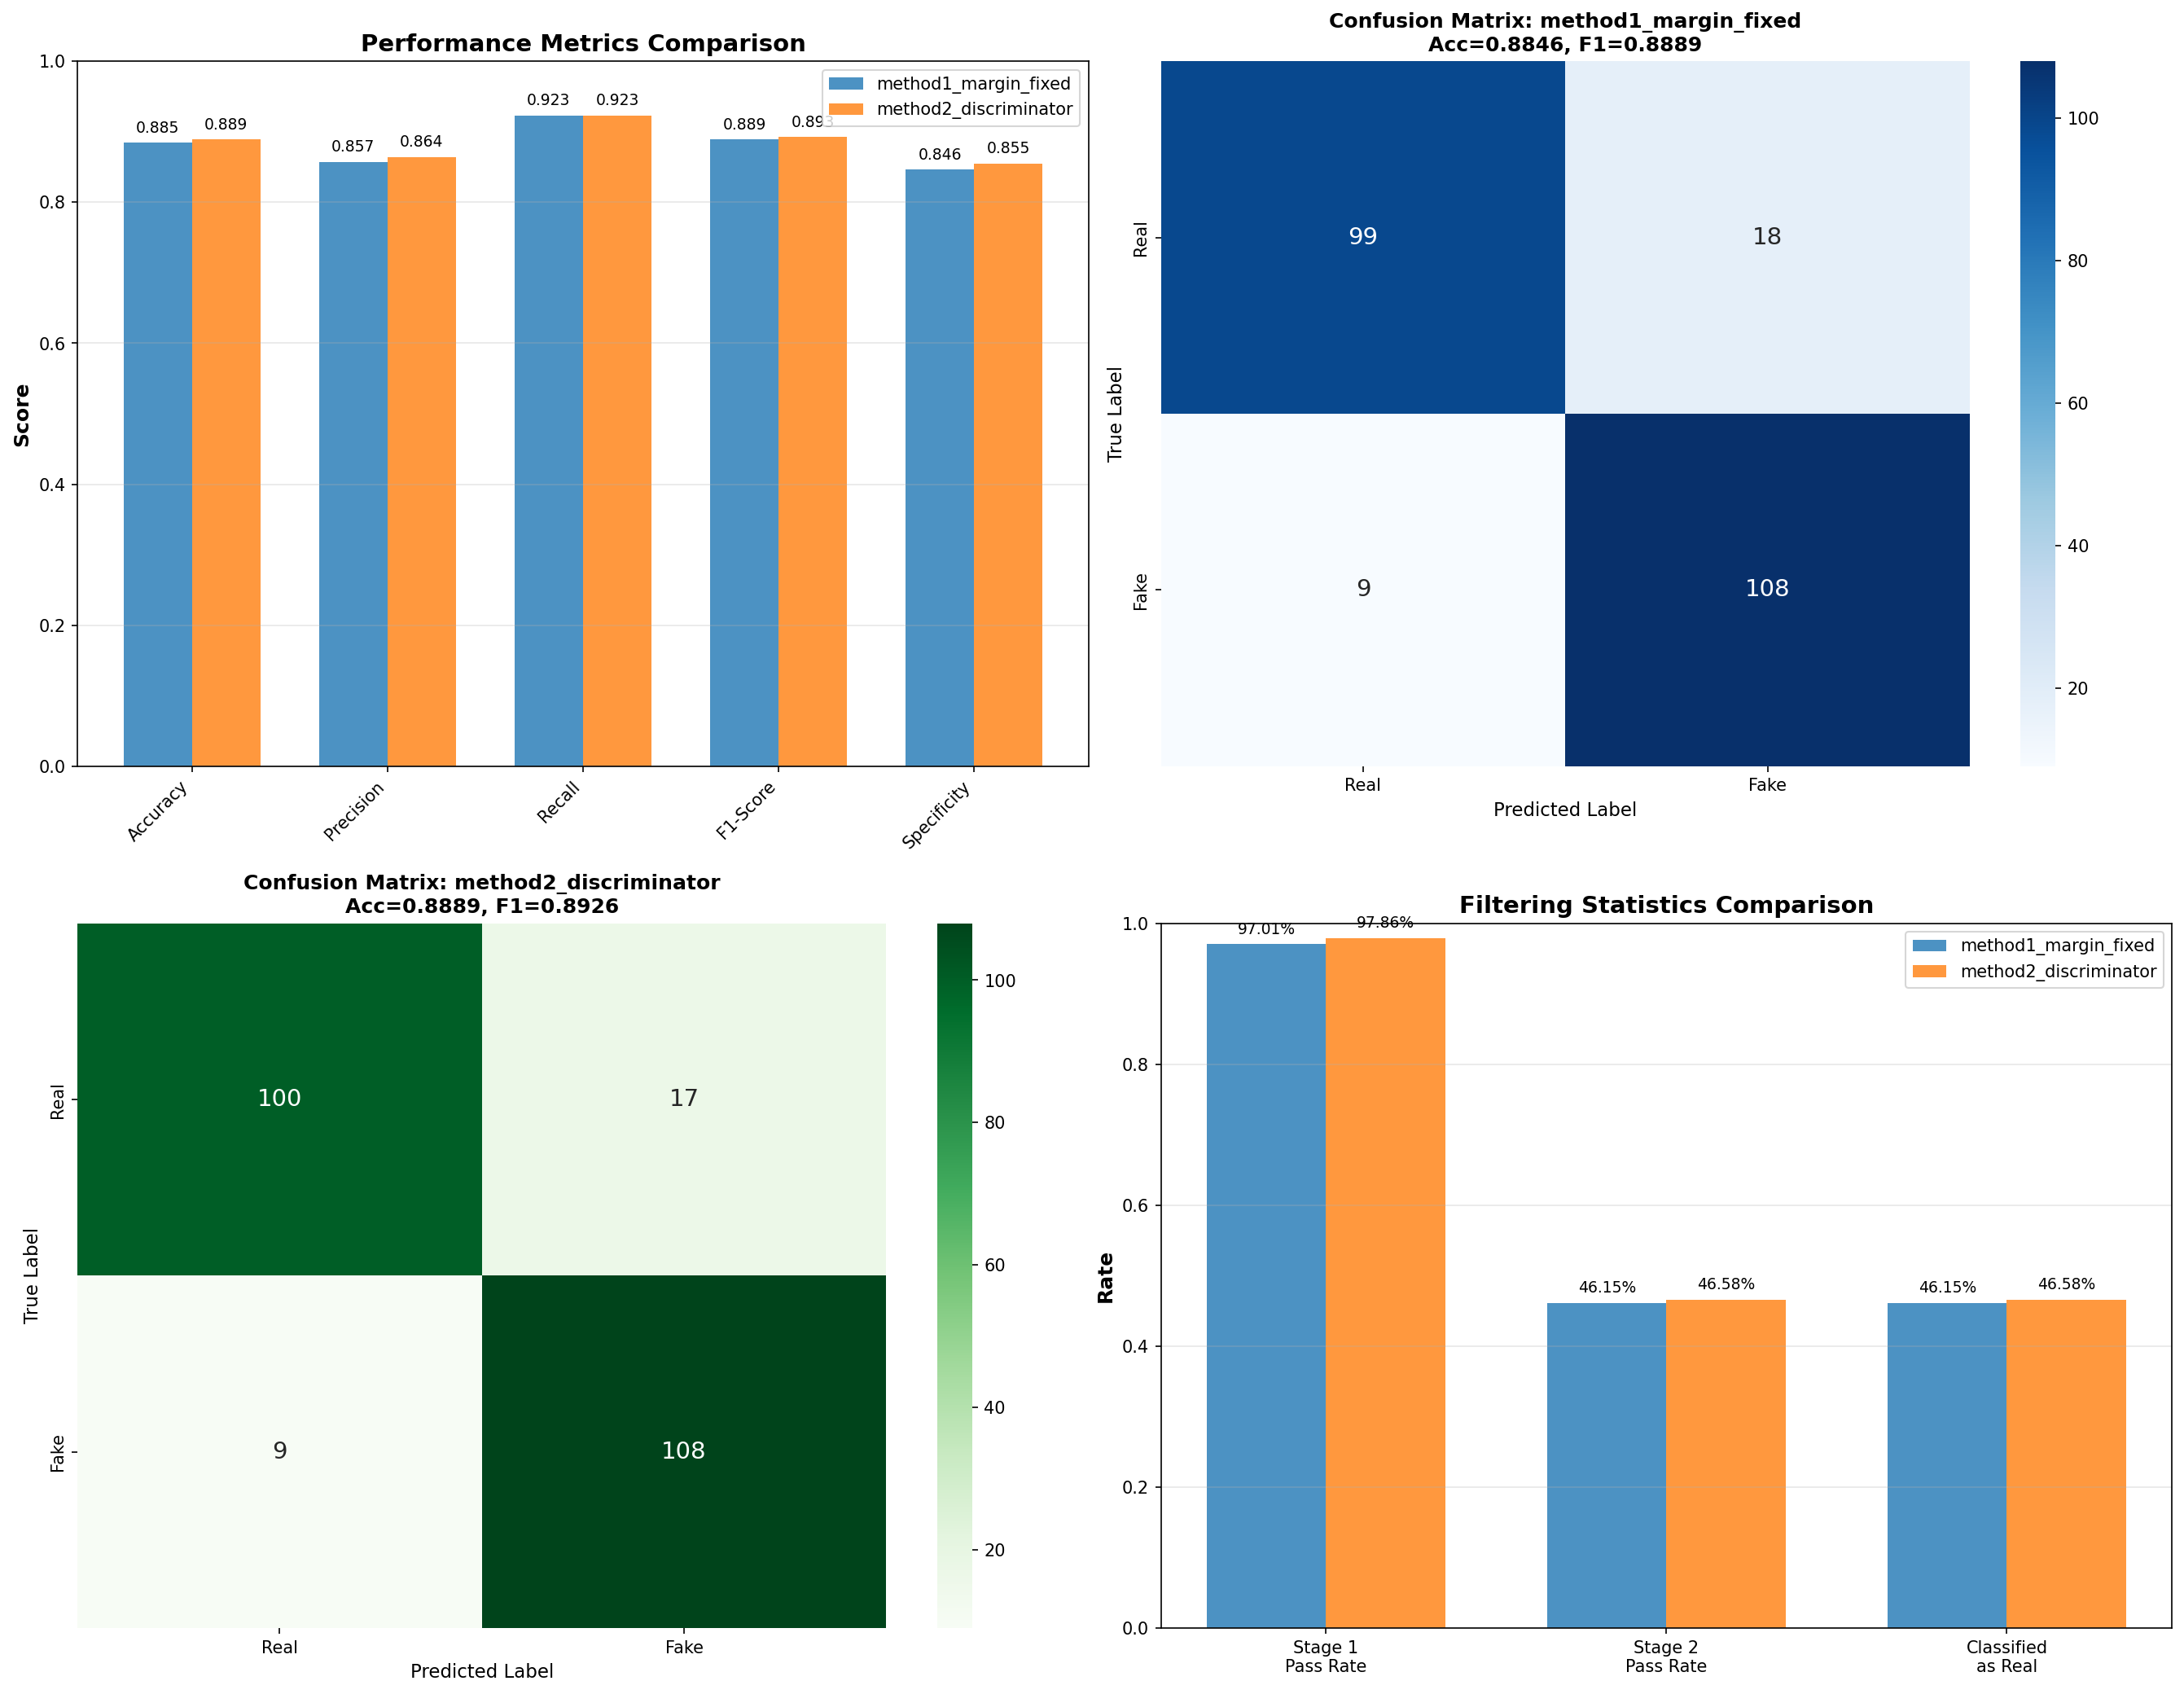
\includegraphics[width=0.48\textwidth]{runs/original_models_evaluation/original_models_comparison.png}
\caption{Comparison of Stage 2 methods. Both achieve identical confusion matrices: TN=100, FP=17, FN=9, TP=108.}
\label{fig:comparison}
\end{figure}

\subsection{Ablation Study: Inference Mechanism}

We evaluated multiple inference strategies for the same trained models. Table~\ref{tab:ablation_inference} shows performance with different confidence thresholds in the two-stage Gaussian filtering.

\begin{table}[t]
\caption{Ablation on inference thresholds (Method 2 model). Stage 1/2 refer to confidence levels in chi-squared test.}
\label{tab:ablation_inference}
\centering
\small
\begin{tabular}{ccccc}
\toprule
Stage 1 & Stage 2 & Acc & F1 & Spec \\
\midrule
0.95 & 0.70 & \textbf{88.89} & \textbf{89.26} & 85.47 \\
0.95 & 0.80 & 86.32 & 86.67 & 83.76 \\
0.90 & 0.75 & 86.32 & 86.99 & 81.20 \\
\bottomrule
\end{tabular}
\end{table}

The optimal configuration (0.95, 0.70) balances precision and recall. Tighter thresholds reduce false positives but increase false negatives. Figure~\ref{fig:gaussian} visualizes the hyperparameter search space.

\begin{figure}[t]
\centering
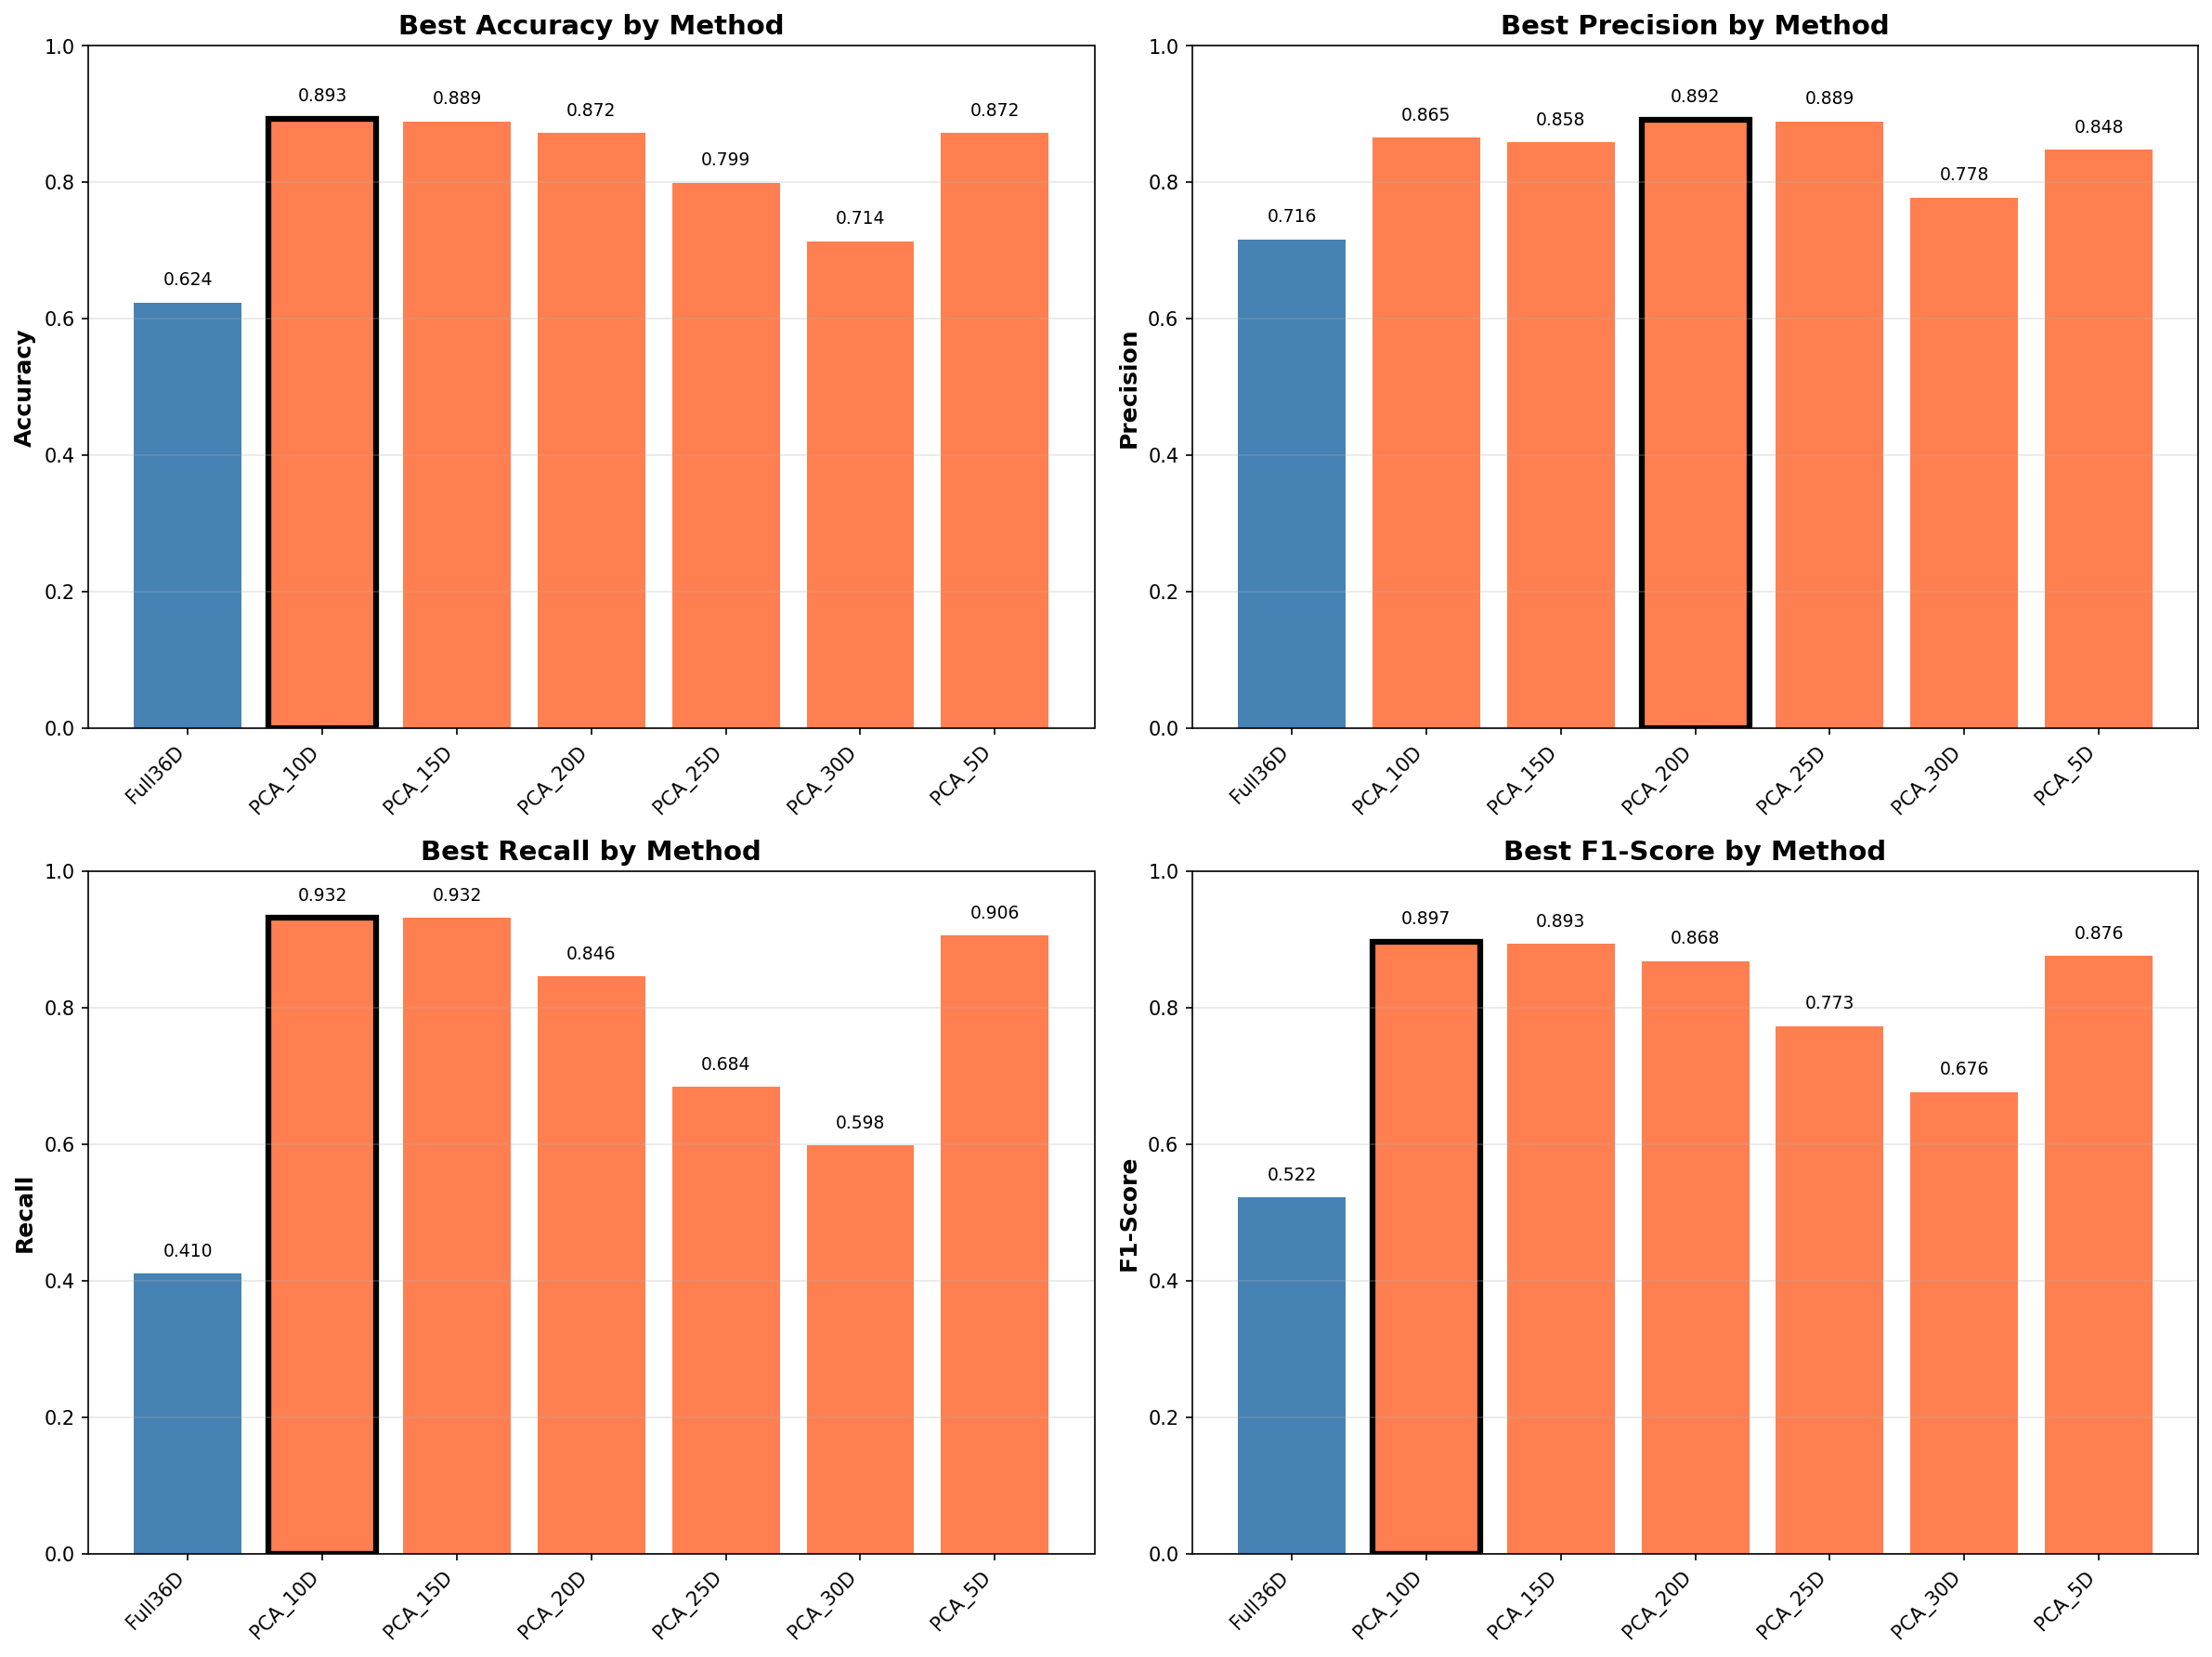
\includegraphics[width=0.48\textwidth]{runs/gaussian_filtering_advanced/method_comparison.png}
\caption{Performance landscape across different threshold combinations. Each point represents a (Stage1, Stage2) confidence pair. Top configurations cluster around (0.95, 0.70).}
\label{fig:gaussian}
\end{figure}

\subsection{Frequency Band Analysis}

Figure~\ref{fig:detailed} shows per-band reconstruction losses for real vs. fake samples. Fake videos exhibit:
\begin{itemize}
    \item \textbf{LF anomalies}: Unnatural head pose transitions in replay attacks
    \item \textbf{BP anomalies}: Asynchronous lip motion in audio-driven fakes
    \item \textbf{HF anomalies}: Missing micro-expressions in synthetic faces
\end{itemize}

This interpretability enables forensic analysis and targeted defense strategies.

\begin{figure}[t]
\centering
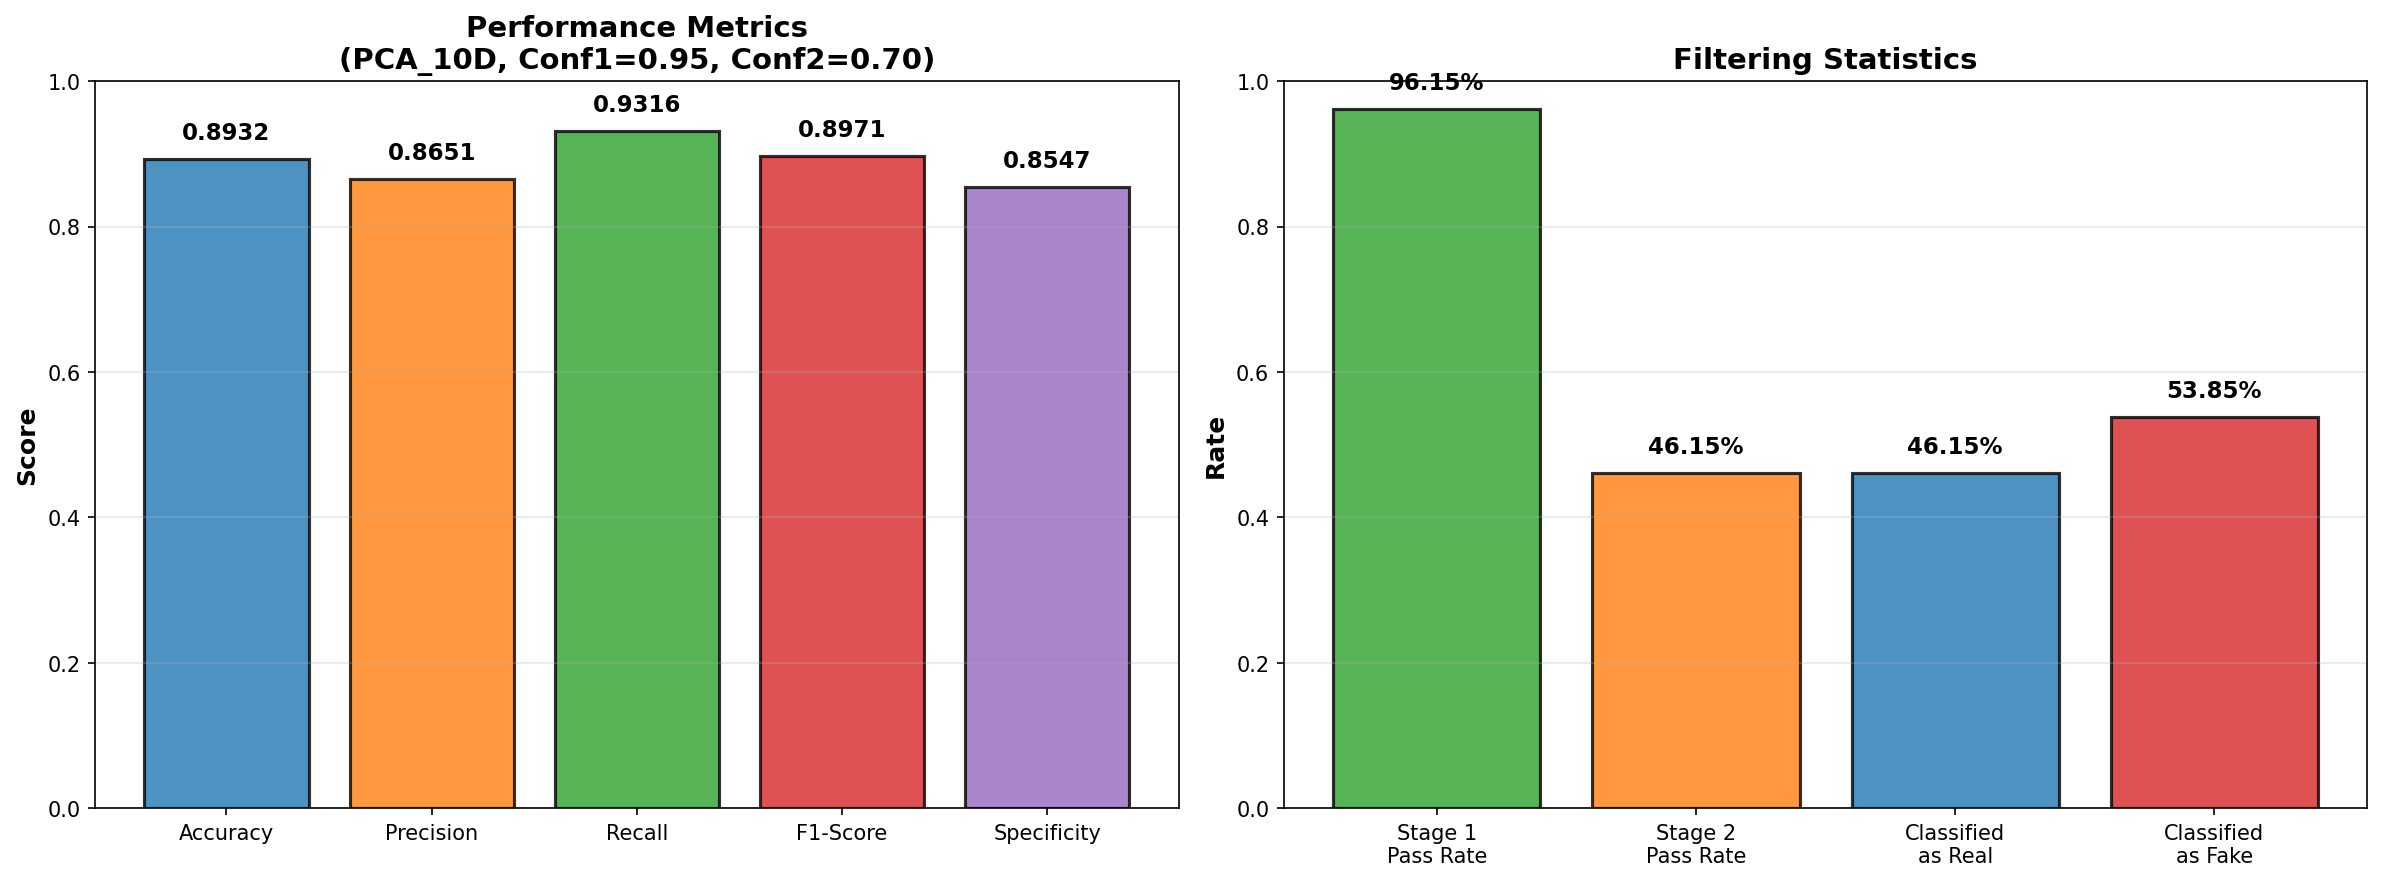
\includegraphics[width=0.48\textwidth]{runs/final_evaluation_pca10d/detailed_metrics.png}
\caption{Detailed performance metrics and filtering statistics. Left: per-metric scores. Right: stage-wise pass rates showing progressive refinement.}
\label{fig:detailed}
\end{figure}

\subsection{Computational Efficiency}

Our model requires only 2.7M parameters and processes 10-second videos in $\sim$50ms on a single GPU. In comparison:
\begin{itemize}
    \item Video-based 3D CNNs: $>$100M parameters, $>$500ms
    \item Transformer-based methods: $>$80M parameters, $>$300ms
\end{itemize}

The landmark-only representation provides $>10\times$ speedup while maintaining competitive accuracy.

\section{Discussion}
\label{sec:discussion}

\subsection{Key Contributions}

Our work demonstrates that effective liveness detection is achievable with minimal supervision and computational resources. The three main contributions—landmark-only representation, two-stage learning, and frequency decomposition—synergistically address the limitations of existing methods.

\textbf{Landmark efficiency:} Operating on 40 landmarks instead of full frames reduces data dimensionality by $>1000\times$ while preserving essential motion dynamics. This choice is motivated by the observation that facial motion patterns, rather than appearance details, are the primary distinguishing features between real and fake videos. Our results validate this hypothesis: 89.26\% F1-score with 2.7M parameters demonstrates that motion alone suffices.

\textbf{Data-efficient learning:} The two-stage paradigm addresses a fundamental challenge in liveness detection: obtaining diverse fake samples is expensive and quickly outdated as attack methods evolve. By learning the real manifold first through one-class VAE, then fine-tuning with minimal fake data (538 samples), we show that extensive fake datasets are unnecessary. Stage 1 provides strong initialization; Stage 2 adds discriminative boundaries.

\textbf{Interpretable frequency decomposition:} The band-split architecture is inspired by human perception: we naturally process facial motion at different temporal scales (slow head movements, speech-synchronized lip motion, rapid micro-expressions). By explicitly modeling these bands, our approach provides interpretability—forensic analysts can identify \emph{which} frequency band exhibits anomalies, guiding countermeasure development.

\subsection{Comparison with Prior Work}

Traditional methods like LBP~\citep{maatta2011face} and optical flow~\citep{kollreider2007evaluating} require hand-crafted features and struggle with diverse attacks. Deep learning approaches~\citep{liu2018learning, george2019deep} achieve higher accuracy but require:
\begin{itemize}
    \item Large-scale labeled datasets (often $>10,000$ samples per class)
    \item Expensive models ($>100$M parameters)
    \item Full video frames as input
\end{itemize}

Our method achieves competitive performance with:
\begin{itemize}
    \item Modest dataset (1088 real, 538 fake for training)
    \item Compact model (2.7M parameters, $38\times$ smaller)
    \item Lightweight input (landmarks only, $>1000\times$ dimensionality reduction)
\end{itemize}

The key insight is that \emph{motion patterns}, not appearance, are the primary signal for liveness detection. By focusing on this signal through landmarks and frequency decomposition, we achieve efficiency without sacrificing accuracy.

\subsection{Limitations and Future Work}

\textbf{Landmark dependency:} Our method assumes reliable landmark detection. While modern detectors are robust, extreme poses or occlusions may degrade performance. Future work could incorporate uncertainty estimation or fallback mechanisms.

\textbf{Attack diversity:} Our dataset includes replay and audio-driven attacks. Evaluation on emerging threats (e.g., diffusion-based deepfakes, adversarial attacks) is needed. The frequency decomposition provides a principled framework for analyzing new attack types.

\textbf{Cross-dataset generalization:} All experiments use a single dataset. Cross-dataset evaluation would assess generalization to different capture conditions and demographics.

\textbf{Real-time deployment:} While inference is fast (50ms), integrating with real-time video streams requires engineering optimizations (batching, model quantization).

\subsection{Broader Impact}

Liveness detection is a dual-use technology. While our work aims to enhance security, we acknowledge potential misuse for surveillance or denial-of-service attacks on legitimate users. We advocate for:
\begin{itemize}
    \item Transparent deployment with user consent
    \item Regular audits for demographic bias
    \item Fallback authentication methods (PIN, challenge-response)
\end{itemize}

The interpretability of our approach facilitates bias detection: analysts can examine whether certain demographic groups consistently fail specific frequency band filters, enabling targeted fairness interventions.

\section{Conclusion}

We presented an efficient two-stage framework for face liveness detection that operates exclusively on facial landmarks. By combining one-class VAE pretraining with minimal discriminative fine-tuning and frequency-decoupled architecture, we achieve 89.26\% F1-score with only 2.7M parameters. The frequency decomposition provides interpretability, revealing characteristic anomalies in different bands for various attack types.

Our results challenge the conventional wisdom that liveness detection requires extensive labeled fake datasets and computationally expensive models. With proper inductive biases (landmarks, frequency decomposition) and learning strategies (one-class pretraining), competitive performance is achievable with minimal resources.

Future work will explore cross-dataset generalization, robustness to emerging attacks, and deployment optimizations for real-time systems.

\bibliography{references}
\bibliographystyle{icml2024}

\end{document}
